\documentclass[11pt]{article}
\usepackage[margin=0.7in]{geometry}
\usepackage{amsmath,amssymb,booktabs,makecell,graphicx,float}
\usepackage[T1]{fontenc}
\begin{document}
\begin{center}
{\Large MICE PMM Variance Estimation}\\[4pt]
{\normalsize Standard MICE PMM with a soft top-k donor-source correction}
\end{center}
\section*{1. Goal and notation}
For each simulation replicate, we create $m$ completed data sets with ordinary \texttt{mice::mice(method = "pmm")}. The completed values and realized donor IDs are exactly those produced by standard MICE PMM. If donor $j$ is selected for recipient $i$, the completed value for $i$ is the observed value of $j$.

The variance problem is that one donor can be used for several recipients. The copied values then share the same observed donor source. A rowwise variance calculation misses this dependence. The correction therefore keeps the realized donor map when forming the completed-data score covariance.

Let $U_i^{(p)}$ be the completed-data analysis score for person $i$ in imputation $p$, let $d_i^{(p)}$ be the imputation-model influence quantity, and let $\tau^{(p)}$ be the completed-data analysis information. For each imputation, the realized donor IDs define a donor-source version of the score, $U_{\Omega,i}^{(p)}$: every recipient who received donor $j$ is assigned to donor source $j$ when the score covariance is formed.

The key donor-reuse component is
\[
  \widehat{\Omega} = \frac{1}{n}\bar U_{\Omega}^{\mathsf T}\bar U_{\Omega},
  \qquad
  \bar U_{\Omega} = \frac{1}{m}\sum_{p=1}^m U_{\Omega}^{(p)}.
\]
Thus, donor reuse affects $\widehat{\Omega}$ through the actual MICE donor labels, not through a simulated approximation to the completed values.

\section*{2. RW variance structure}
The estimator follows the Robins--Wang form. With $\bar d=m^{-1}\sum_p d^{(p)}$, $\widehat{\alpha}=(nm)^{-1}\sum_p d^{(p)\mathsf T}d^{(p)}$, and $\widehat{\tau}=(nm)^{-1}\sum_p\tau^{(p)}$, define
\[
  \widehat{\Delta} = \widehat{\Omega} + \widehat{\kappa}\widehat{\alpha}\widehat{\kappa}^{\mathsf T}
  + \frac{\widehat{\kappa}\bar d^{\mathsf T}\bar U_{\Omega} + (\widehat{\kappa}\bar d^{\mathsf T}\bar U_{\Omega})^{\mathsf T}}{n},
  \qquad
  \widehat V = \frac{1}{n}\widehat{\tau}^{-1}\widehat{\Delta}\widehat{\tau}^{-\mathsf T}.
\]
The remaining task is to construct the PMM part of $\widehat{\kappa}$ in a way that reflects the matching rule while preserving standard MICE PMM draws.
\clearpage
\section*{3. Soft top-k working probability}
For a missing recipient $i$ and an observed donor $j$, standard PMM selects uniformly from the recipient's nearest-$k$ donor set. That selection rule is discontinuous as the PMM regression coefficient $\psi$ changes. We use a smooth probability only for the variance score.

Let $l_j$ and $u_j$ be the lower and upper prediction-score boundaries for donor $j$ to enter a nearest-$k$ set. Let $\eta_i$ be the recipient's PMM prediction and $s_i$ be the fitted posterior prediction standard deviation. The working probability is
\[
 q_{ij}(\psi) = \frac{1}{k}\left[
 \Phi\left\{\frac{u_j-\eta_i}{s_i}\right\} -
 \Phi\left\{\frac{l_j-\eta_i}{s_i}\right\}
 \right].
\]
Its derivative moves the donor predictions, recipient prediction, and the two membership boundaries together. The probability is used to calculate a differentiable PMM score. It does not replace MICE matching: MICE still chooses one donor uniformly from its realized nearest-$k$ set and copies that donor's observed value.

\section*{4. Rao--Blackwell donor-source term}
Let $U_{ij}^{(p)}$ denote the counterfactual analysis score if recipient $i$ were assigned donor $j$ in imputation $p$. Directly using the observed donor outcome in this term is noisy. We instead use its conditional expectation,
\[
 G_{ij}^{(p)} = E\left\{U_{ij}^{(p)} \mid X_j, \text{recipient information}\right\},
 \qquad
 \widehat{\kappa}_{\mathrm{RB}} = \frac{1}{nm}\sum_{p=1}^m\sum_i\sum_j
 G_{ij}^{(p)}\frac{\partial q_{ij}^{(p)}}{\partial\psi}.
\]
For the RW linear setting, $G_{ij}^{(p)}$ is obtained by replacing the donor outcome with its fitted normal-model mean. For the GS setting, $G_{ij}^{(p)}$ integrates the downstream score under that fitted normal PMM model using fixed Gauss--Legendre quadrature.

The derivative applies only to $q_{ij}$. We do not add $q_{ij}\,\partial G_{ij}/\partial\psi$, because MICE matching conditions on observed donor values; the variance score describes how donor selection changes, not a newly generated donor outcome.
\clearpage
\section*{5. Calculation sequence and reported comparisons}
For each imputed data set, the calculation is:
\begin{enumerate}
\item Run standard MICE PMM and record its completed values and realized donor IDs.
\item Fit the completed-data analysis model and obtain $U^{(p)}$, $d^{(p)}$, and $\tau^{(p)}$.
\item Construct $q_{ij}^{(p)}$ and $\partial q_{ij}^{(p)}/\partial\psi$ from the fitted PMM prediction model.
\item Form $\widehat{\kappa}_{\mathrm{RB}}$, retain the actual donor-source score in $\widehat{\Omega}$, and assemble $\widehat V$ with the RW formula.
\end{enumerate}
The tables report PMM-corrected/Rubin-PMM pairs. The point estimate is the same under both methods because both use the same completed MICE PMM data. They differ only in the estimated variance and hence in coverage. Coverage of $\beta^\ast$ uses the Monte Carlo mean estimate as the target and assesses variance calibration. Coverage of $\beta_0$ uses the data-generating coefficient and therefore also reflects finite-sample bias.

All completed cells below use 2,500 Monte Carlo replications. The figure shows exact 95\% binomial Monte Carlo intervals for each coverage estimate.
\clearpage
\begin{center}
{\Large MICE PMM Simulation Results}\\[4pt]
{\normalsize Current standard-MICE PMM results; 2,500 Monte Carlo replications per completed cell}
\end{center}
\vspace{4pt}
\begin{table}[H]
\centering
\scriptsize
\setlength{\tabcolsep}{2.6pt}
\begin{tabular}{rlrrrrrr}
\toprule
$m$ & \makecell{Imputation\\model} & \makecell{Mean\\estimate} & Bias &
\makecell{Empirical\\SD} & \makecell{Mean estimated SE\\Proposed/Rubin} &
\makecell{Coverage $\beta^\ast$\\Proposed/Rubin} &
\makecell{Coverage $\beta_0$\\Proposed/Rubin} \\
\midrule
5 & PMM ($k=5$) & 0.856 & -0.037 & 0.133 & 0.131 / 0.168 & 0.946 / 0.982 & 0.925 / 0.968 \\
 & PMM ($k=10$) & 0.848 & -0.045 & 0.133 & 0.131 / 0.168 & 0.948 / 0.977 & 0.919 / 0.964 \\
 & PMM ($k=20$) & 0.838 & -0.053 & 0.137 & 0.131 / 0.172 & 0.940 / 0.978 & 0.910 / 0.958 \\
 & PMM ($k=30$) & 0.823 & -0.074 & 0.135 & 0.130 / 0.172 & 0.938 / 0.982 & 0.892 / 0.952 \\
\addlinespace[2pt]
25 & PMM ($k=5$) & 0.857 & -0.035 & 0.127 & 0.126 / 0.165 & 0.949 / 0.987 & 0.928 / 0.979 \\
 & PMM ($k=10$) & 0.848 & -0.044 & 0.126 & 0.125 / 0.166 & 0.950 / 0.988 & 0.926 / 0.981 \\
 & PMM ($k=20$) & 0.837 & -0.060 & 0.124 & 0.124 / 0.167 & 0.946 / 0.989 & 0.909 / 0.975 \\
 & PMM ($k=30$) & 0.820 & -0.071 & 0.132 & 0.124 / 0.167 & 0.932 / 0.986 & 0.884 / 0.963 \\
\addlinespace[2pt]
50 & PMM ($k=5$) & 0.856 & -0.035 & 0.122 & 0.125 / 0.164 & 0.950 / 0.993 & 0.931 / 0.982 \\
 & PMM ($k=10$) & 0.848 & -0.043 & 0.123 & 0.124 / 0.165 & 0.952 / 0.992 & 0.924 / 0.988 \\
 & PMM ($k=20$) & 0.834 & -0.058 & 0.127 & 0.124 / 0.167 & 0.938 / 0.987 & 0.906 / 0.976 \\
 & PMM ($k=30$) & 0.817 & -0.071 & 0.127 & 0.123 / 0.167 & 0.939 / 0.989 & 0.893 / 0.970 \\
\addlinespace[2pt]
100 & PMM ($k=5$) & 0.855 & -0.036 & 0.121 & 0.124 / 0.164 & 0.953 / 0.994 & 0.935 / 0.988 \\
 & PMM ($k=10$) & 0.848 & -0.042 & 0.123 & 0.124 / 0.165 & 0.951 / 0.991 & 0.932 / 0.982 \\
 & PMM ($k=20$) & 0.833 & -0.057 & 0.127 & 0.123 / 0.166 & 0.949 / 0.991 & 0.912 / 0.977 \\
 & PMM ($k=30$) & 0.821 & -0.068 & 0.127 & 0.124 / 0.167 & 0.945 / 0.990 & 0.894 / 0.968 \\
\bottomrule
\end{tabular}
\caption{GS setting, $n=2000$. Proposed/Rubin pairs are PMM-corrected/Rubin-PMM. Bias is the Monte Carlo mean estimate minus the data-generating coefficient.}
\end{table}
\clearpage
\begin{figure}[H]
\centering
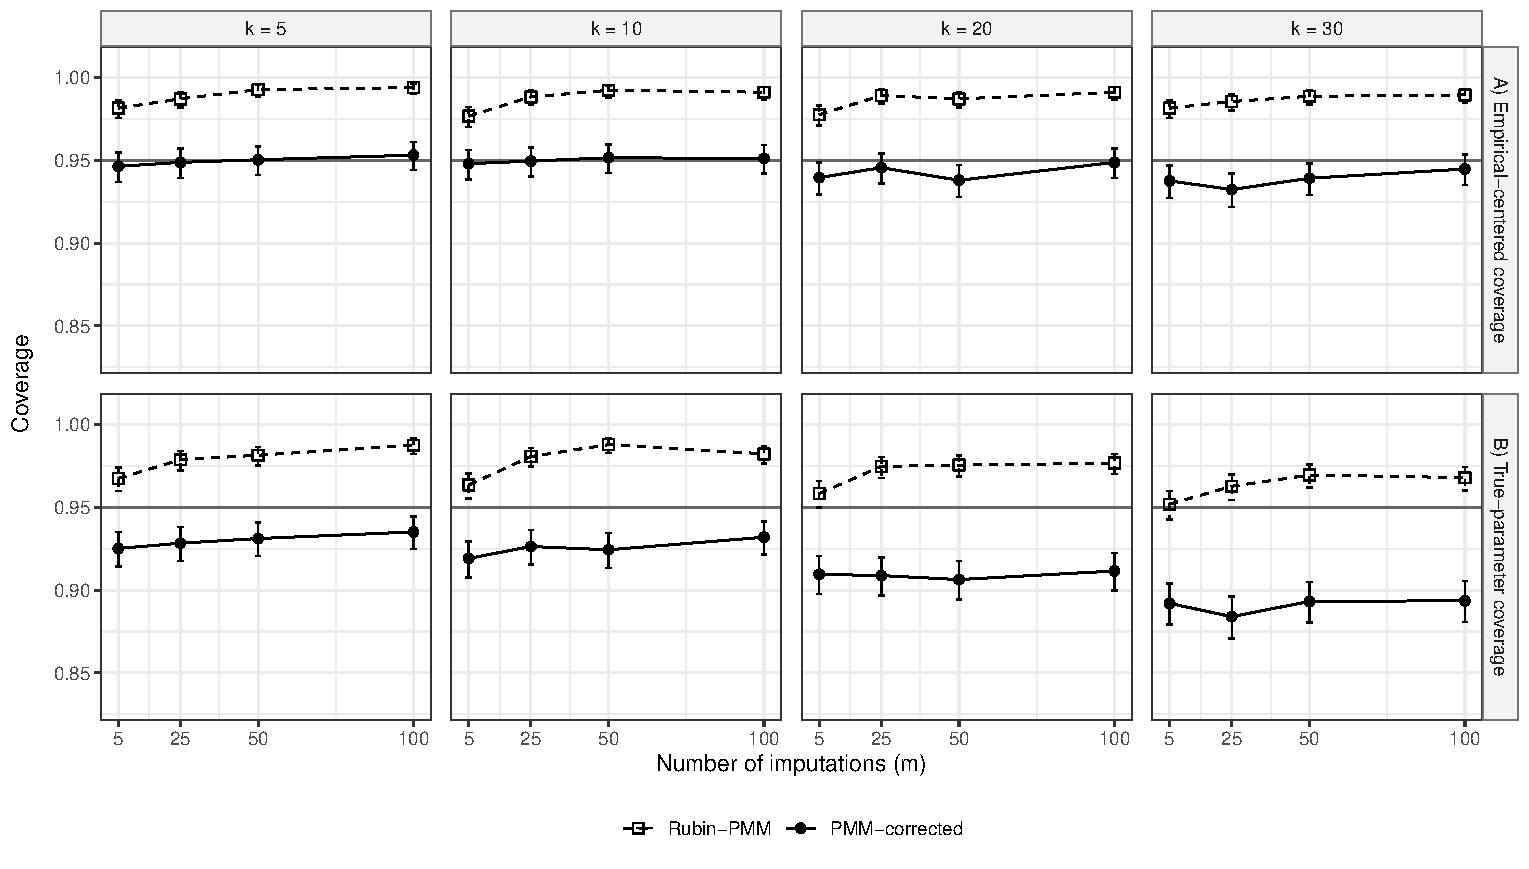
\includegraphics[width=\textwidth]{coverage.pdf}
\caption{GS coverage for standard MICE PMM. Error bars are exact 95\% binomial Monte Carlo intervals.}
\end{figure}
\clearpage
\begin{table}[H]
\centering
\scriptsize
\setlength{\tabcolsep}{3.2pt}
\begin{tabular}{llrrrrrr}
\toprule
Scenario & \makecell{Imputation\\model} & \makecell{Mean\\estimate} & Bias &
\makecell{Empirical\\SD} & \makecell{Mean estimated SE\\Proposed/Rubin} &
\makecell{Coverage $\beta^\ast$\\Proposed/Rubin} &
\makecell{Coverage $\beta_0$\\Proposed/Rubin} \\
\midrule
R1 & PMM ($k=5$) & 1.000 & -0.000 & 0.063 & 0.061 / 0.061 & 0.947 / 0.937 & 0.947 / 0.937 \\
R2a & PMM ($k=5$) & 0.997 & -0.003 & 0.064 & 0.063 / 0.049 & 0.947 / 0.856 & 0.945 / 0.854 \\
R2b & PMM ($k=5$) & 0.996 & -0.004 & 0.047 & 0.046 / 0.073 & 0.948 / 0.996 & 0.949 / 0.995 \\
R2c & PMM ($k=5$) & 1.000 & 0.000 & 0.063 & 0.062 / 0.046 & 0.945 / 0.834 & 0.944 / 0.833 \\
R3a & PMM ($k=5$) & 0.939 & -0.061 & 0.039 & 0.038 / 0.038 & 0.950 / 0.952 & 0.633 / 0.638 \\
R3b & PMM ($k=5$) & 1.688 & 0.688 & 0.054 & 0.054 / 0.057 & 0.944 / 0.954 & 0.000 / 0.000 \\
\bottomrule
\end{tabular}
\caption{RW setting, $n=1000$, $m=50$, and $k=5$. Each scenario has 2,500 Monte Carlo replications. Proposed/Rubin pairs are PMM-corrected/Rubin-PMM.}
\end{table}
\clearpage
\begin{table}[H]
\centering
\scriptsize
\setlength{\tabcolsep}{3.2pt}
\begin{tabular}{llrrrrrr}
\toprule
Scenario & \makecell{Imputation\\model} & \makecell{Mean\\estimate} & Bias &
\makecell{Empirical\\SD} & \makecell{Mean estimated SE\\Proposed/Rubin} &
\makecell{Coverage $\beta^\ast$\\Proposed/Rubin} &
\makecell{Coverage $\beta_0$\\Proposed/Rubin} \\
\midrule
R1 & PMM ($k=5$) & 0.980 & -0.020 & 0.165 & 0.151 / 0.153 & 0.912 / 0.916 & 0.909 / 0.912 \\
R2a & PMM ($k=5$) & 0.992 & -0.008 & 0.165 & 0.153 / 0.120 & 0.921 / 0.832 & 0.921 / 0.832 \\
R2b & PMM ($k=5$) & 0.967 & -0.033 & 0.126 & 0.119 / 0.183 & 0.929 / 0.992 & 0.924 / 0.992 \\
R2c & PMM ($k=5$) & 0.993 & -0.007 & 0.166 & 0.152 / 0.110 & 0.909 / 0.800 & 0.910 / 0.800 \\
R3a & PMM ($k=5$) & 0.936 & -0.064 & 0.100 & 0.096 / 0.098 & 0.933 / 0.942 & 0.881 / 0.891 \\
R3b & PMM ($k=5$) & 1.664 & 0.664 & 0.153 & 0.136 / 0.139 & 0.915 / 0.916 & 0.016 / 0.016 \\
\bottomrule
\end{tabular}
\caption{RW setting, $n=150$, $m=20$, and $k=5$. Each scenario has 2,500 Monte Carlo replications. Proposed/Rubin pairs are PMM-corrected/Rubin-PMM.}
\end{table}
\end{document}
